\documentclass{report}
\usepackage{fullpage}
\usepackage{graphicx}
\usepackage{pdfpages}
\usepackage{amsmath}
\graphicspath{{figures/}}
\title{Design of An Innovative, Highly Maneuverable, Stealthy Unmanned Underwater Vehicle with ISR Capabilities }
\setlength{\parindent}{4em}
\author{Andrew Blancarte\\ Ketton James\\ Brian Martin\\ Abraham Paucar\\ Ben Saletta}
\date{\today}
\renewcommand{\chaptername}{Phase}
\renewcommand{\bibname}{References}
\begin{document}
\maketitle
\tableofcontents
\listoffigures
\chapter{Propulsor Development, SHEILA-D}
\section{Overview}
SHEILA-D stands for Subaquatic Hydrodynamicaly propelled Explorer Implementation Los Angeles - Demonstrator. The driving force behind the development of this unmanned underwater vehicle is the innovative propulsion system. This system was the foundation of the first phase of development, a proof of concept for this screw based propulsion system. As this phase was a deliverable for a Machine Design Class there is a detailed overview of this phase included in appendix A. 
\section{Constraints}
As this initial design was part of a class project there were many constraints that came along with it. The primary constraint was time. The project was completed, from design to testing, in 35 days to meet the deadline imposed by the academic calender. There were also significant cost constraints because this phase was funded completely out of the personal funds of the members involved. The constraints eliminated several custom manufacturing techniques due to extensive lead times and costs. This led to the final construction consisting mainly of parts shaped from hardware store components.
\section{Design}
The initial design phase took the first 5 days in which the foundational fluid mechanics, the drive train and power calculations were completed in these days. Further redesign was included in with the manufacturing process when the aforementioned constraints restricted the construction of the device as designed.
\subsection{Fluids Calculations}
The fluids calculations were an important part of the initial design because of the roll they played in moving the device through the water. To complete these calculations the device was broken into two sections. First the cylinder holding the screw and second the cone used to accelerate the fluid. For the cylinder an assumption was made that a constant force would be imparted to the fluid along the surface of the screw blades. This constant force would act on the fluid mass between the vanes therefore, assuming a constant density, the vanes would provide a constant acceleration along this section. With a known length of the cylinder and this calculated acceleration the speed of the fluid exiting the cylinder was calculated. Conservation of momentum was then applied to the fluid as it passed through the final cone and nozzle giving the final thrust force of the propulsion system. These calculations were plugged into an Excel spreadsheet and various geometries were iterated through to find the optimal configuration. A more detailed walk through of the fluids analysis is included in appendix A.
\subsection{Drive Train}
The fluids calculations provided a value for the required torque and angular velocity. The drive train was designed to meet both of these criterion. The major difficulty with the drive train in this design was transmitting the torque from the motors to the external shell. To solve this problem and provide sufficient torque two motors were fitted with gearboxes then mated to the sun gear in a planetary gear set that transmitted the torque out to the rotating cylinder as seen in Figure 1.1. The planetary gear system was 3D printed to minimize cost and manufacturing time.
\begin{figure}[h]
\centering
\includegraphics[width=15cm]{"Section View"}
\caption{Drive Train Design Section View}
\end{figure}
\subsection{Power Supply}
These motors required a significant amount of current at a constant 12 volts. These requirements went into the power design calculations and searches for sufficient batteries. A single 12 volt lithium battery was selected due to its high current discharge, compact form, and high capacity characteristics. The design of the power supply was integrated into the design of the drive train due to the important relationship between the easily available motors and batteries for a reasonable operational time. The power supply had to fit between the two motors and is shown as a black box in Figure 1.1.
\section{Construction}
The construction of this device was completed in a very short time span using commercial off the shelf components. This involved PVC pipes of various diameters, cutting and thermoforming sheets of acrylic, and fastening components with traditional fasteners as well as epoxy. As the construction proceeded difficulties were discovered and the design was adjusted to compensate for these problems. One of the major difficulties was the manufacture of the helix screw. This was solved by thermoforming cut acrylic then filling gaps created in the vanes with waterproof tape. Other adjustments and quick fixes were applied through out the process. The construction was a challenge to complete within the time frame at an acceptably low cost.  
\section{Testing}
Once construction was completed the device needed to be tested to confirm that the propulsion system did indeed propel the device through the water. To do the testing properly the vehicle was taken to the Puddingstone reservoir at dawn and ran along the deck of a boat dock. It took a few tests to get the device operational and, while the vehicle could not be set off on its own at this stage, it pumped a significant amount of water though the body and out the cone and nozzle assembly. Many things were learned about the design during the testing session and made note of for future design. The major lessons were that the assumptions that were made in the fluid calculations were wrong and that without control surfaces the vehicle would reach an equilibrium rotation state where the outermost cylinder would rotate and counter the rotation of the center cylinder. 
\chapter{Summer Research and Testing}
During the summer of 2014 the group members of Team UV did not entirely part ways for three months. The group decided that it would be in the best interest of the group and design itself to meet twice a month where each member would give presentation on standard material along with research they have found during the two week period between meetings. These meetings started in June of 2014 and ended when the 2014 Fall period started, September 2014.  Each of the meetings held were roughly five to seven hours long. The format of the presentations were standardized however each member provided their own research and information. Presentation format can be found in appendix B. In the summer of 2014 Team UV spent roughly 240 hours as a group towards the senior project itself. That number includes research done outside of the meeting along with the meetings themselves. The PowerPoint presentations contained three sections.
\section{Open Mind}
The group was given a situation/problem that has or could happen in the world we live in today and each member had to give insight or propose a solution to the problem/situation. Each member were asked to provide their solution along with reasoning  as to why their solution would be efficient. Since Team UV are composed of mechanical engineering undergraduates, the solutions based on the prompts were required to use some aspect of engineering. For example, one open mind prompt addressed the issue that many people in developing countries lack the access to power. The group was asked if they were tasked with developing an inexpensive “do it yourself” power generation system for use in a 3rd world country, what kind of engineering considerations might you take into account. The idea behind the open mind prompt was to keep the group members mind engaged during the break and keep that engineering mentality sparked. Also, this prompt was to have the members think outside the box and to aid in developing creative/innovative ideas for use in the senior project design.
\section{Well-Read}
Members were asked to look into articles/publications and present something they found to be interesting, innovative, advancements, etc. The articles were not limited to strictly the engineering field however it was recommended.  Articles presented from the group ranged from next generation wind turbines to theory behind the process of suction eating of fish. The idea of the well-read was to give insight to the group of remarkable advancements in science and technology throughout the world.
\section{Presentation}
The presentation was an open ended section which allowed for each member to present some research they did during the two week period between meetings. The research was required to aid in the design of the senior project in areas such as theory, analysis, design, controls, manufacturing, and/or testing. Research in CLT propellers, computational fluid dynamics, Arduino coding, wake turbulence, underwater designs and coatings, power management, component selection for marine research, smart ducts, submarine design/research, and many others. 
\section{Summer Research Summaries}
\subsection{Shark Skin}
\begin{figure}[h]
\centering
\includegraphics[width=5cm]{"Shark Skin"}
\caption{Close up of Shark Skin}
\end{figure}
Sharks move very efficiently thanks to the characteristics of their skin.  Anything but smooth, shark skin has individual scales, called dermal denticles, with narrow passages that reduce friction drag and accelerate the flow along its length.  These scales also flex and realign to reduce biofouling which can negatively affect flow over the body.

\subsection{Vantablack}
\begin{figure}[h]
\centering
\includegraphics[width=5cm]{"Vantablack"}
\caption{Vantablack on Aluminum Substrate}
\end{figure}
Surrey NanoSystems has engineered a new super-black material called Vantablack.  This material composed of “Vertically Aligned Carbon Nanotube Arrays” absorbs 99.965\% of incident light.  Photons are allowed into the material and are then blocked and trapped from leaving.  This material is already in high demand for space and stealth applications. 

\subsection{Cephalopod Skin}
\begin{figure}[h]
\centering
\includegraphics[width=5cm]{"Cephalopod Skin"}
\caption{Cephalopod Skin}
\end{figure}
Two teams of researchers from Rice University and MIT were tasked with developing material which could replicate the camouflaging abilities of cephalopods.  The class of mollusks which include squid, possess skin that can manipulate its own color and texture.  Rice University engineering a rigid aluminum nanorod display panel which displays an intense color spectrum.  MIT, on the other hand, created a flexible display that can change color and texture but with limited color spectrum.

\subsection{Waterproofing Sensors}
\begin{figure}[h]
\centering
\includegraphics[width=4cm]{"Potting"}
\includegraphics[width=6cm]{"Conformal Coating"}
\caption{Potting and Conformal Coating}
\end{figure}
Using sensors underwater with a strict budget takes a bit of creativity.  Two popular methods used by hobbyists and professionals alike are: Potting and Conformal Coating.  Potting is the method of filling an electronic assembly with a solid or gelatinous compound such as a thermosetting plastic or silicone.  This blocks water and increases shock resistance.  Conformal Coating offers the same benefits of potting but is lighter and non-permanent which allows for reworking.
\subsection{Arduino}
\begin{figure}[h]
\centering
\includegraphics[width=5cm]{"Arduino UNO"}
\caption{Arduino Uno Microprocessor}
\end{figure}
Microprocessing is made accessible to all thanks to companies like Arduino.  Boards housing everything from input and output terminals to a microprocessor can link the electrical world to the physical world.  Users start out controlling the lighting sequencing of LED’s to eventually controlling more advanced mechanical systems.  Topics presented to the team include LED control, reading data from sensors, and ways to expand the factory limitations of Arduino boards.  
\subsection{CFD and Python}
Computational Fluid Dynamics, CFD, is a powerful tool for the analysis of fluid behavior. The computational techniques used to break down the navier-stokes equations have applications that stretch beyond the realm of fluid dynamics and allow the modeling of many non linear mathematical phenomena within a computational environment. This presentation was an introduction to the ideas behind CFD and the way that an analysis could be written using the Python coding language.
\subsection{Physical Understanding of Fluids Equations and their Application to CFD}
To apply any of the fundamental fluids equations to a device a physical understanding of the meaning behind the mathematics is crucial. This presentation addressed four different ways to address a fluids problem. First analysing a stationary control volume and applying conservation of mass equations to the borders. Secondly selecting a moving control volume of fixed mass and applying conservation of momentum equations to the borders. Thirdly selecting an infinitely small particle and analyzing the fluid that passes through it. Or finally selecting an infinitely small particle and analyzing its path through the fluid. This allows for the analysis of any problem from a variety of different perspectives.
\subsection{Optimal Design of an Archimedes screw}
As the device that we are manufacturing depends upon a screw similar to the original archimedes screw it was important that we analyze the methods used to optimize the design of one of these screws.\cite{Rorres00} This introduced the idea of breaking a design down into dimensionless variables that dictated the ratio of the size of components and reduced the amount of unknown variables. These dimensionless numbers were then varied and efficiencies were calculated providing the final, most efficient design ratios.
\subsection{Tom's Effect}
Fish are covered with mucus primarily to cover wounds and promote healing, however this mucus also causes Tom’s Effect. This is when a high molecular weight polymer is released into a fluid stream it makes the fluid remain laminar for longer because the polymers line up with the streamlines in the fluid. This requires the fluid to use more energy to break the streamlines and become turbulent. With fish this allows them to travel through the water with significantly less drag than they otherwise would have had to overcome. The could be applied to any underwater vessel to provide increased fuel efficiency and stealth.
\subsection{WHOI Acoustic Modem}
 Underwater communications have been a long standing challenge because radio waves attenuate rapidly in water. A possible method for communication between several underwater vehicles or even between a vehicle and its home base is an acoustic modem. These work by emitting modulated sound waves that carry data through the water. Due to the high speed of sound through water these methods of communication become practical. 
\subsection{CLT Propellers}
\begin{figure}[h]
\centering
\includegraphics[width=5cm]{"CLT"}
\caption{Contacted and Loaded Tip Propellers}
\end{figure}
Fundamentally the goal of the Contracted and Loaded Tip (CLT) propeller is to improve open water efficiency.  This means that the tip on the propeller reduces the velocities of water entering the propeller disk which, in turn, reduces the hydrodynamic pitch angle.  This reduction of hydrodynamic pitch angle and induced velocities results in many advantages.  To list a few, CLT propellers achieve higher top speeds, greater thrust, smaller optimum propeller diameter, better maneuverability, inhibits cavitation and tip vortices (resulting in less noise, less vibrations, lower pressure pulses, and lower area ratio
\subsection{Smart Duct}
\begin{figure}[h]
\centering
\includegraphics[width=5cm]{"Smart Duct"}
\caption{Thrust Vectoring Smart Duct}
\end{figure}
A Smart Duct is a deformable shroud that changes the direction of flow of the propeller wash to provide a direct steering force to the vehicle.The duct itself is an electrically actuated structure that is covered by a flexible hydrodynamically smooth sheathing whose primary movers are a set of high strength Nickel-Titanium SMA actuator cables.  Shape memory alloys (SMA) make this deformable Smart Duct a reality. Testing has proven flow turning angles of up to 15 degrees at thrust levels of operational submarines is possible with this technology.  These results may directly affect the design of future marine vehicles by reducing (and possibly eliminating) the use of control surfaces for maneuvering.
\subsection{Vortex Generators}
\begin{figure}[h]
\centering
\includegraphics[width=5cm]{"Vortex Generators"}
\caption{Vortex Generators on the Wing of a Fighter Jet}
\end{figure}
For relatively blunt objects like a sphere or wing on a plane the overall drag decreases when the boundary layer becomes turbulent because turbulent flow allows the boundary layer to follow the surface closer which decreases the overall wake region.  The larger this wake region is the more you see chaotic flow separation and adverse pressure gradients that can be catastrophic on aircraft because the flow separation can cause them to stall.Vortex generators can be found on the wings of aircraft and even on some high performance cars.  With vortex generators there is an exchange between high energy momentum and lower energy momentum by tripping laminar flow into turbulent which allows the boundary layer to remain attached over a greater length of the wing chord or car profile which results in a thinner wake region and smaller adverse pressure gradient on the rear of the object which lowers the pressure drag.  This allows for many benefits like lowering the stall speed, improving stability and control during maneuvering, and decreasing the turning radius.
\subsection{Wanda II}
\begin{figure}[h]
\centering
\includegraphics[width=5cm]{"Wanda II"}
\caption{Wrasse-inspired Agile, Near-shore, Deformable-fin Automation}
\end{figure}
Researchers have turned to nature for inspiration trying to model a UUV that uses flapping fins to maneuver through difficult underwater environments.  Many fish species use articulation of the pectoral fins to produce appropriate forces and moments propel themselves through the water and to react to dynamic changes in flow, physical obstacles, and wave forces near the shore. A four-fin UUV named WANDA-II (Wrasse-inspired Agile Near-shore Deformable-fin Automaton) is the 2nd generation of this alternative propulsion UUV. These fins are capable of producing thrust vectors in multiple directions through changes in curvature and stroke angle. All this is in the attempt to replicate the high level of controllability that fish species have near shore and in shallow water environments. A four-fin UUV could be deployed in a variety of missions including harbor monitoring and protection, hull inspection, and covert shallow water operations. 
\subsection{Control Surface Basics}
\begin{figure}[h]
\centering
\includegraphics[width=5cm]{"Pitch Roll Yaw"}
\caption{Representation of Euler Angles}
\end{figure}
Control Surfaces are moveable surfaces on wings that allow for maneuverability for both air and marine vehicles. Typically when control surfaces deflect they change the trailing edge of the wing which in turn changes the angle of attack. Angle of attack is the angle of between the wing chord (leading edge to trailing edge) to the Relative Airflow or free air flow (RAF). The amount of lift a wing produces is more a function of the angle of attack rather than the shape of the airfoil (cross section of the wing).The primary control surfaces on an airplane are ailerons (which controls roll/pitch), elevators (which controls pitch), and the rudder (which controls yaw).
\subsection{Materials and Stealth}

“…five major underwater vehicle requirements.  The two key issues are technical feasibility and stealth.  The third important issue is survivability.  Fourth, and equally important is the need to successfully deliver a payload.  And finally, all of these attributes regardless of importance, must be considered within a framework of cost.” (Submarine Technology for the 21st Century).\par
\begin{figure}[h]
\centering
\includegraphics[width=5cm]{"Submarine Stealth"}
\caption{Sonar Detection of a Submarine}
\end{figure}
Research was done into submarine hull materials and what we could learn from them for our project within the framework of parameters such as weight/speed, strength/depth capability, stiffness, corrosion resistance, magnetic signature, machinability/formability, fatigue resistance, thermal properties, electrical properties, and acoustic properties.  Research was conducted into steel, titanium, aluminum, composites (Carbon Fiber-, Titanium-, and Glass Fiber-Reinforced Polymers), and general polymers.\par
\par Stealth was investigated with regards to passive control (active control was not looked into owing to the impracticality with regards to the scope/scale of our project).  Passive control research centered firstly on the effect of polymeric bodies and polymer secretion on the hydrodynamic boundary layer, skin friction, wake field, general turbulence, vortices, and hydrodynamic noise generation.  The next direction for passive control was towards acoustic stealth via the use of anechoic materials (with sublayers for absorbing sonar waves, damping and decoupling of internal signal waves, and transmission layers for areas with intentional signal emission/transmission) and machinery “raft” beds (for vibration and noise damping), including attenuation ranges, elastomeric viscoelastic mechanical models, porosity effects (on attenuation, damping, and chemical stability), the correlation of relaxation modulus with temperature, signal frequency, and thermal transitions, and chemical stability (hydrolytic stability and water absorption).
\subsection{Funding}
Research was conducting with regards to sources of project financial support.  Options looked into included National Science Foundation (NSF) and Department of Defense (DoD) grants, innovation competition awards, (financial, material, product, and service) sponsorships (and the possible development of a sponsorship brochure) and donations, and online crowdsourcing.  The final decision was to use crowdsourcing for the majority of the fundraising and to look for sponsors and donors whenever possible.  Specific companies further researched for sponsorship, donation, or discount included Proto Labs, Rapid Machining, Quick Parts, Solid Concepts, and the Cal Poly Pomona Southern California Engineering Technologists Association (SCETA).\par
Websites looked into for hosting the crowdsourcing campaign included KickStarter, Indiegogo, RocketHub, and GoFundMe.  Aspects considered included campaign type [Flexible (keep what you raise) vs. Fixed (all or nothing)], timeline, campaign durations, processing/collection timelines and fees, donor rewards, website demographics (aimed at technical or artistic people), website traffic, and connectivity with social media.\par
At this time, the team also created social media accounts with Facebook, Instagram, and Twitter in order to help spread awareness of both the fundraising campaign and the website (which was created through WordPress.com after consideration and research into the same basic considerations as for the fundraising campaign, with the addition of website cost, domain ownership, and customization considerations).
\subsection{Testing}
Research was also conducted into both industry standard marine vehicle testing (mostly the use of tow tanks and the specific parameters often focused on with industry testing, i.e. the Admiralty Coefficient) and testing that we could perform. \par
\begin{figure}[h]
\centering
\includegraphics[width=5cm]{"Test Tank"}
\caption{Underside of a Boat in a Tow Tank}
\end{figure}
The first future test highlighted for our project included powered movement testing with stabilizing surfaces (for cancelling out torque transfer and rotation transmitted to the outer body) and a distributed weight belt (for inducing neutral buoyancy) with the parameters of interest of water speed, thrust, and flow field visualization.  Other test ideas consisted of battery run time tests, sealing tests, and small scale concept tests (i.e. using a cut open 2L bottle, cone to fit into the bottle, and swirling motion to determine the most efficient exit flow type through measuring drain time and waterproofing small DC motors and connecting them to vane shells of various geometries inside submerged tubes).
\subsection{Thrust Augmentation}
Research was conducted into Zone I (hull and pre-shaft inlet sections), Zone 2 (fluid working section), and Zone III (outlet section) thrust augmentation devices, their implementation, and how they influence propulsive efficiency, flow separation, turbulence, propulsor swirl (pre-swirl and post-swirl) (and thus flow equalization), cross flow minimization (and thus bilge vortices), effective thrust, shaft vibrations, wake field magnitude and distribution, open water efficiency, energy recovery, propeller hub vortices, conversion of rotational kinetic energy to directional flow, hydrodynamic lift, and lift-drag ratio.  Devices researched include:
\begin{itemize}
\item Zone I: Wake equalizing ducts, asymmetric sterns, Grothues spoilers, stern tunnels, semi- or partial ducts, reaction fins, Mitsui Integrated Ducted Propulsion Units, and Hitachi Zosen Nozzles.
\item Zone II: Increased diameter-low RPM propulsors, Grim Vane Wheels, propellers with end-plates, CLT propulsors, and propeller cone fins.
\item Zone III: Rudder-Bulb fin systems and additional thrusting fins.
\end{itemize}
\begin{figure}[h]
\centering
\includegraphics[width=5cm]{"Thrust Augmentation"}
\caption{Thrust Augmentation on the Hull of a Ship}
\end{figure}
\indent Research was also conducted into the effect of combination of devices with the conclusion that most combinations were not possible due to one device removing the regime utilized by the other, while a select few combinations led to good benefits.
\subsection{Owl Stealth}
\begin{figure}[h]
\centering
\includegraphics[width=8cm]{"Owl Stealth"}
\caption{Wing Features on an Owl that Provide Stealthy Flight}
\end{figure}
Research was conducted into the mechanisms by which owls derive their acoustic stealth, with the goal of better understanding the turbulent eddies and their amplification/scattering from the trailing edges of wings (natural or man-made) and how biomimicry might be able to change the way our control surfaces might affect our stealth (acoustic or flow signature).  Research centered on the profiles, material properties (most importantly stiffness), geometry, and surface roughness of the leading edge, mid-wing section, and trailing edge.\par
It was determined that the trailing edge is the dominant noise source on wings and that owl wing stealth was mainly the result of use of leading and trailing edge tubercles and flexible, porous trailing edge material.  Tubercles were to be a future feature of our vehicle's control surfaces, time permitting.
\subsection{Submarine Hydrostatics}
\begin{figure}[h]
\centering
\includegraphics[width=8cm]{"Submarine Hydrostatics"}
\caption{Center of Buoyancy and Center of Mass of a Submarine}
\end{figure}
Research was conducted into ship and submarine hydrostatics in the surfaced, diving/surfacing, and submerged states.  Key factors considered included state of buoyancy, reserve of buoyancy, trim, configuration and use of main ballast tanks (internal and external), free flood spaces, margin ballasts, variable ballasts, superstructures, flexible bag ballasts with flotation collars, freeboard, and a pressure hull.\par
\indent Methodologies for buoyancy calculation were researched heavily for both intact and damaged vessel states, surface (static), surfacing/diving (transition), and submerged (static) states, conditions of flotation, and disturbance response for small and large values of sway, yaw, surge, heave, and (the most complex case) heel/roll.\par
\indent Some specific takeaways included the final decision with regards to buoyancy control system and flood/vent hole design (i.e. location and use of a grill if requiring a large hole in order to disrupt noise, vibration, and drag caused by the flood/vent hole(s)).
\subsection{Submarine Design Process}
\begin{figure}[h]
\centering
\includegraphics[width=5cm]{"Submarine Design"}
\caption{Design Considerations for Underwater Vehicles}
\end{figure}
Research was conducted into the submarine design process as presented in Concepts in Submarine Design, 2s (Burhcer).  This design process is shown below, with the accelerated modifications for our time-sensitive project shown in red.\par
Note: Bolded text in the following paragraphs highlights the applicability to our project. Specific topics focused on included  role designation \textbf{(ISR)} [and subsequent subrole \textbf{(perform ISR in a covert manner within a variety of environments while retaining high stealth, maneuverability, elevated speeds, and sufficient battery life)]}, development of operational requirements \textbf{(specifics of speed, maneuverability, battery life, stealth characteristics, etc. requirements)}, concept studies (with key parameters of size, cost, payload, performance), feasibility studies (and system material requirements) \textbf{(development of weight, space, and power budgets for various sub-systems in design)}, \textit{design for build} (detailed systems, subsystems, arrangements, configurations, specifications, etc. \textbf{(management of previously developed budgetary allocations with deliverables relating to structures, arrangements, hydrodynamics, subsystems, hydrostatics (both surface and submerged), etc.)}, and production design \textbf{(final vehicle design)}.
\subsection{Buoyancy Control}
A research article contained information related to buoyancy control of a semiautonomous underwater vehicle and design orientation. The orientation of the design determined what the application of the vehicle. For example, if the design were to be horizontal resembling a manta ray, its use would be for towing and exploration at lower depths. However, due to this orientation it has a higher chance of getting stuck in densely populated sea vegetation or between underwater rocks. If the orientation were to be vertical, resembling a fish, its use would be for a remote controlled mode and towing as well. The vertical orientation makes it easier to maneuver in densely populated sea vegetation. The buoyancy control mechanism contained two compressed air tanks connected to two separate balloons. The air would be released into the balloon when the vehicle needed to raise and the air would be released the vehicle needed to be lowered.
\subsection{Underwater Coatings}
Cathodic protection is used in a vary of underwater applications. Cathodic Protection (CP) is a technique used to control the corrosion of a metal surface by making it the cathode of an electrochemical cell. A simple method of protection connects the metal to be protected to a more easily corroded "sacrificial metal" to act as the anode. The sacrificial metal then corrodes instead of the protected metal. The sacrificial metal that has been corroded provides a protective surface to prevent the base material from being corroded. Alocit by the A\&E group is an coating that is used for underwater applications. It is one of three coatings that meet the specs of the US Army Corps of Engineers.
\subsection{Currents}
\begin{figure}[h]
\centering
\includegraphics[width=5cm]{"Currents"}
\caption{Currents and Overall Fluid Transport}
\end{figure}
Currents are broken down into two types, surface and deep water. Deep water currents usually occur more than 400 meter (~1300 feet) under the surface of the water. The water movements are caused by differences in water density known as Thermohaline circulation. Deep water currents are much slower than surface currents but they move much more water due to water density increase deeper in the sea. Surface currents are due to the Coriolis Effect. The Coriolis Effect occurs due to the rotation of the earth, the circulating air is deflected resulting in curved paths. The wind’s curved path drags on the water’s surface, causing it to move in the direction the wind is blowing. The Ekman Spiral is a consequence of the Coriolis Effect.
\section{TeamUV.org}
Establishing TeamUV.org was the obvious next step after a Summer filled with professional growth and academic exploration.  Not only was the website about the current progress of the team’s senior project but also about inspiring interest in STEM and facilitating monetary support.  Topics covered range from fluid dynamics, robotics, and biomimicry to shining light on what engineering is and how it impacts the world.  Inspired by websites often visited by Team UV members, posts were uploaded various times throughout the week to keep followers intrigued without feeling overwhelmed.  Well Reads, Presentations, and Open Minds were set to be posted on Tuesdays, Thursdays, and Sundays, respectively.  Each post was written by a team member according to a set schedule set for months in advance.  A list of website postings can be found in Appendix .  Team UV also made sure that the website was linked with companion Facebook, Twitter, Instagram, and GoFundMe accounts.\par
\indent Team UV.org went live on July 31, 2014 with a welcome post about the site, the project, and ways to help the team’s fundraising campain.  The site instantly created buzz pulling in 122 views and 38 visitors the first month.  After gaining a steady following from all around the world including 87 countries, TeamUV.org achieved a best month of 670 views and 518 unsubscribed visitors in January 2015.  To date, the site has gained a steady, recurring base of 84 subscribed followers that actively visit and participate in leaving comments for the team.\par
\indent Aside from weekly posts, visitors to the site can also find team member biographies giving background about personal interests, academic experiences, and professional work.  Those looking to sponsor the team’s efforts with donations or equipment are also able to give directly on the site, follow a  link to the Team UV GoFundMe site, or contact the them directly.  

\section{Summer Testing}
Along with delving into Summer research pertaining to many aspects of engineering design, Team UV also performed a couple of tests.  Another trip to Sailboat Cove was made to test the benefits of attaching control surfaces to Sheila-D.  Spring Quarter testing resulted in the formation of a free exit jet but minimal displacement of the vehicle.  Due to stacking inefficiencies with material availability, available manufacturing methods, and unaddressed torque transfer issues, Sheila-D was in need of support.  Scrap square pieces of aluminum flashing were roughly attached to the sides of the propulsor which controlled the overturning moments caused by torque transfer in the device.  This resulted in linear travel along the dock, verifying the projects potential.\par
Testing the importance of the exit cone was also performed during the summer session.  2-liter soda bottles were modified to resemble the flow through Sheila-D.  Water was passed through the model’s nozzle. with and without an exit cone, and discharge times were recorded.  The use of the exit cone was verified by the faster exit times of the cone-equipped soda bottle.  Tests were also performed as to the effects of pre-swirl into the nozzle caused by the vane shell.  Tests using modified soda bottles showed promising results as the water look to discharge out the nozzle faster with pre-swirl but were eventually ruled inconclusive.  Controlling the swirl of the exiting water was difficult to accomplish giving the tests poor repeatability.\\
\chapter{Final Prototype Design and Manufacture, DORY}
\section{Lessons Learned}
\section{Subsystem Decomposition}
\subsection{Propulsor}
\subsubsection{Control Volumes}
In order to perform our internal fluids analysis on the propulsor with the goal of optimizing the vane shell, we had to treat the problem as a basic fluid mechanics problem and start with the same foundational elements of all fluid mechanics problems; we had to define some control volumes.\par
Before jumping right into defining our control volumes, we had to identify the parameters of interest to us; of these, we highlighted four main parameters that were to be treated as unknowns:
\begin{enumerate}
\item Inlet velocity at the front of the propulsor $v_1$
\item Pressure at the end of the vane shell and prior to the nozzle $P_2$
\item Exit velocity at the rear of the nozzle $v_3$
\item Thrust force produced by the vehicle $F_T$
\end{enumerate}
Additionally, these values would be evaluated at three main state points:
\begin{itemize}
\item The free stream inlet region ahead of the propulsor $(1)$
\item The interface between the back of the vane shell and the start of the nozzle/cone$(2)$
\item The exit region immediately behind the nozzle $(3)$
\end{itemize}
To properly solve for these four unknowns, we needed four equations and thus we developed four control volumes $(A, B, C, D)$, each with a distinct equation associated with it as will be shown below.  Once we had these four equations developed, the plan was to use an iterative programming technique to solve the four equations for the four unknowns, thus yielding the parameters necessary for finding the basic performance characteristics associated with the propulsor.  This will be discussed in greater detail in the programming section of the report that follows.\par
As will be seen below, the basic types of equations utilized in the analysis consisted of the conservation of energy and the conservation momentum; conservation of mass was not utilized as it did not yield any helpful information with regards to the problem solving process.\par
\begin{equation}
\frac{P_i}{\gamma}+\frac{v_i^2}{2g}+h_{L_{i-f}}=\frac{P_f}{\gamma}+\frac{v_f^2}{2g}+h_{s_{i-f}}
\end{equation}
\begin{equation}
\Sigma F=P_iA_i+\dot{m}v_i+P_fA_f-\dot{m}v_f-F_T+F_D=ma
\end{equation}
\paragraph{Control Volume A}
For control volume $A$, the energy equation was adopted, with the unknowns of $v_1$ and $P_2$.
\begin{figure}[h]
\centering
\includegraphics{"Ctrl Volume A"}
\caption{Schematic of Control Volume A}
\end{figure}
\begin{figure}[h]
\centering
\includegraphics{"Eqn A"}
\caption{Simplified Energy Equation for Control Volume A}
\end{figure}
As can be seen, the inlet pressure term was set equal to zero, as this was taken to be gage pressure since it is simply the free-stream hydrostatic field pressure.  The two elevation terms also cancel, because even if the propulsor was stood up vertically, the change in elevation would only be one to three feet (this length had yet to be determined), which would be negligible; additionally, the vast majority of the time, the vehicle would be travelling at roughly zero angle of attack (and therefore would not have a change in elevation from front to back of the propulsor).\par
This leaves a few terms remaining; $g$ is simply the gravitational acceleration (32.2 $\frac{ft}{s^2}$), $\gamma$ is simply the specific weight of the fluid (water; 62.4 $\frac{lb}{ft^3}$), $v_1$ is the inlet velocity (an unknown, as defined earlier), $P_2$ is the pressure at the end of the vane shell (another unknown, as defined earlier), $v_2$ is the velocity at the end of the vane shell, $h_{L_{1-2}}$ is the energy loss term from front to back of the vane shell, and $h_{s_{1-2}}$ is the shaft input energy term from front to back of the vane shell.\par
In order to reduce this equation further to the original two unknown values we wished to solve for, we had to come up with equations for the $v_2$, $h_{L_{1-2}}$, and $h_{s_{1-2}}$ terms.\par
Using the fact that $v_2$ represents the maximum speed our vane shell could get the fluid moving without slip, we defined the maximum vane shell axial fluid speed to be equal to the angular velocity times the effective screw pitch associated with the vane shell, which is a function of the average radius (average between the base radius, or outside radius of the cylinder onto which the vanes attach and the maximum radius, or the radius to the tips of the vanes) and the angle of twist of the vanes:
\begin{equation}
v_2=\omega P;p=\frac{2\pi r_{avg}}{\tan(\theta)}
\end{equation}
The next term is the head loss term along the length of the vane shell ($h_{L_{1-2}}$); this term would normally include both major (due to friction) and minor losses (due to components), but since there is not any major bends/corners/etc., the minor losses were neglecting, reducing the head loss term to that of purely major loss.
\begin{equation}
h_{L_{1-2}}=f\frac{L}{D_h}\frac{v^2}{2g}
\end{equation}
The velocity ($v$) used above would be taken as the average between the free stream velocity ($v_1$, an unknown) and the maximum/end of vane shell velocity ($v_2$) and thus would require iteration in the program.  The length of the vane shell ($L$) would be assumed in the iteration at different values in order to determine the desired unknown values over a range of lengths.  The hydraulic diameter ($D_h$) would be determined for each set of iterations on the basis of assumed vane shell geometry (just like the length), through the formula:
\begin{equation}
D_h=\frac{4A}{P}
\end{equation}
where $A$ is the area of the flow (determined by finding the sum of all inter-vane flow areas, as restrained by vanes on either side of the flow, the rotating cylinder on the bottom of the flow, and the stationary body cylinder on the top of the flow).  Lastly, the friction factor ($f$) was determined as the Darcy-Weisbach friction factor through the use of the Swamee-Jain approximation of the Colebrokk-White equation:
\begin{equation}
f=\left\{\begin{array}{ll}
\frac{64}{Re}&:Re\leq2000~~Laminar\\
.25[\log(\frac{\epsilon}{3.7D_h}+\frac{5.74}{Re^{.9}})]^{-2} &:Re>2000~~Turbulent\\
\end{array}
\right.
\end{equation}
\begin{equation}
Re=\frac{v_{avg}D_h}{\nu}
\end{equation}
where $\eta$ is the material roughness,$Re$ is the Reynolds number as defined in equation 3.7, and $\nu$ is the kinematic viscosity of the fluid.
Lastly, the shaft head ($h_{s_{1-2}}$) was taken as:
\begin{equation}
h_{s_{1-2}}=\frac{T\omega}{\gamma Q}
\end{equation}
where $\omega$ is the rotational speed (as defined earlier), $\gamma$ is the specific weight (as defined earlier), $Q$ is the volumetric flow rate (the product of the average velocity and the flow area, as both defined earlier), and $T$ is the torque.  Torque was defined as a fluid torque through its relation to the rotational speed of the screw-like vane shell and the twist of the path of water (more details about this may be found in the appended original Phase I report calculations, appendix A):
\begin{equation}
T=\frac{(r_avg\omega)^2}{2g}\gamma A \cos(\Phi)(r_avg)
\end{equation}
With all of these equations developed, it becomes apparent that the original energy equation (after substitution of assumed geometry and iterated angular velocities) has been reduced to two unknowns ($v_1$ and $P_2$), albeit in a highly intertwined fashion.
\paragraph{Control Volume B}\par
For control volume $B$, the energy equation was again adopted, this time with the unknowns of $P_2$ and $v_3$.
\begin{figure}[h]
\centering
\includegraphics{"Control Volume B"}
\caption{Schematic of Control Volume B}
\end{figure}
\begin{figure}[h]
\centering
\includegraphics{"Eqn B"}
\caption{Simplified Energy Equation for Control Volume B}
\end{figure}
Once again, elevations cancel, one pressure (this time the exit pressure) interfaces with the hydrostatic pressure field and is thus set to zero gage pressure, and this time the shaft input energy term is set to zero because we are now beyond the vane shell and only have stationary components.  $P_2$ (an unknown) is defined the same as before, $v_2$ is the maximum/end of vane shell velocity (as defined earlier), and $v_3$ (also an unknown) is the free jet exit velocity, as defined earlier.  This just leaves the head loss term, which unlike before now contains both major (due to friction and calculated the exact same way as before, except between points 2 \& 3, rather than 1 \& 2) and minor losses (due to components).  The minor losses were modeled through use of the following general minor loss equation:
\begin{equation}
h_{L_{2-3}(minor)}=K\frac{v_{avg}^2}{2g}
\end{equation}
where $K$ is the component loss coefficient, which in this case was taken conservatively as the worst case non-reentrant scenario entrance loss coefficient ($K=0.5$), although our situation would never come near this scenario.
\begin{figure}[h]
\centering
\includegraphics[width=8cm]{"Nozzel Minor Losses"}
\caption{K values for Minor Losses due to Diameter Change}
\end{figure}
With all of these equations developed, it becomes apparent that the original energy equation (after substitution of assumed geometry and iterated angular velocities) has been reduced to two unknowns ($v_3$ and $P_2$), albeit in a highly intertwined fashion.
\paragraph{Control Volume C}\par
For control volume $C$, the momentum equation was adopted, with the unknowns of $P_2$, $v_3$, and the thrust force $F_T$.
\begin{figure}[h]
\centering
\includegraphics{"Control Volume C"}
\caption{Schematic of Control Volume C}
\end{figure}
\begin{figure}[h]
\centering
\includegraphics{"Eqn C"}
\caption{Simplified Energy Equation for Control Volume C}
\end{figure}
$P_3$ is once again set to zero gage as it is the hydrostatic field pressure, drag force ($F_D$) is assumed zero for the small nozzle section, and acceleration ($a$) is taken to be zero due to the assumption that steady state velocity (no acceleration) has been reached.  $P_2$, $v_2$, and $v_3$ are defined as before and the thrust force ($F_T$) is one of the desired unknowns.  $A_2$ is the area of the annular flow region between the circular nozzle and the circular pressure hull/start of cone (not pictured).  This just leaves the mass flow rate ($\dot{m}$), which is the product of the average velocity from point 2 to 3, the density of the fluid (water), and the effective flow area as previously discussed.\par
Once again, with all of these equations developed, it becomes apparent that the original momentum equation (after substitution of assumed geometry and iterated angular velocities) has been reduced to three unknowns ($v_3$, $P_2$, and $F_T$).
\paragraph{Control Volume D}
For control volume D, the momentum equation was adopted, with the unknowns of $v_1$, $v_3$, and the thrust force $F_T$.
\begin{figure}[h]
\centering
\includegraphics{"Control Volume D"}
\caption{Schematic of Control Volume D}
\end{figure}
\begin{figure}[h]
\centering
\includegraphics{"Eqn D"}
\caption{Simplified Energy Equation for Control Volume D}
\end{figure}
Just as before, $P_1$ and $P_3$ are both taken to be zero gage due to their interfacing with the hydrostatic field pressure and the acceleration is set to zero due to assumed steady state operation; also as seen previously, $v_1$, $v_3$, and $F_T$ are all desired unknowns and mass flow rate is calculated the same as before, with the average velocity being taken between points 1 and 3.  The only new term being introduced here is the drag force ($F_D$).\par
The drag force is calculated with the classic algebraic form of the drag force equation:
\begin{equation}
F_D=0.5\rho C_D v^2 A
\end{equation}
where $\rho$ is the fluid (water) density, $v$ is the average velocity between points 1 and 3, $A$ is the reference area (in this case taken as the outermost circular cross-sectional area of the body cylinder), and $C_D$ is the drag coefficient, which has been taken conservatively to be $1.2$.\par
One last time, with all of these equations developed, it becomes apparent that the original momentum equation (after substitution of assumed geometry) has been reduced to three unknowns ($v_1$, $v_3$, and $F_T$).
\paragraph{Integration of Control Volumes}
With all of these control volumes and the associated equations, it can be seen that we have developed four equations (the ones boxed in red in the previous sections) as a function of four desired unknowns ($v_1$, $P_2$, $v_3$, $F_T$).  As can be seen the system of four equations is statically determinant with the right assumptions made, but is nonlinear in nature and highly inter-dependent, requiring a very complex computer program to be written in order to integrate the four equations together to solve for the desired unknowns, as will be discussed in the next section.  A summary of the desired unknowns for each control volume is provided below.
\begin{enumerate}
\item Control Volume A (Energy Equation from 1 to 2): $v_1$ and $P_2$
\item Control Volume B (Energy Equation from 2 to 3): $P_2$ and $V_3$
\item Control Volume C (Momentum Equation from 2 to 3): $P_2$,$v_3$, and $F_T$
\item Control Volume D (Momentum Equation from 1 to 3): $v_1$, $v_3$ and $F_T$
\end{enumerate}

\subsubsection{MatLab Code}
The mathematical model rendered through the above control volume analysis still contained many unknowns. With the above equations the relationship between these unknowns could be determined, however finding the optimal value of each of the 5 geometrical dimensions and the one dynamic variable would have required exhaustive iterations and guess work. To facilitate the design process and ensure optimal design a program was written in the MatLab coding environment that would cycle through ranges of each of these variables, creating every possible combination of designs and rank them on an efficiency. This would allow for the most efficient design to be selected.\par
The majority of the variables in question described the geometry of the propulsor. To reduce the complexity of the design some variable were designated before the program began. The length of the nozzle was fixed to 5 inches, providing a reference size so that the most efficient design would still have a reasonable package size. The number of vanes was set to 5, in previous iterations of the program a value of 5 vanes commonly populated the highest efficiency and therefore it was set, freeing up processing time for more volatile variables. The outer radius, inner radius, length, angle of the vane helix, and nozzle radius were allowed to vary. Each variable had to have a range to vary within because without a finite range the program would loop infinitely. The maximum outer radius was set to 5 inches, the minimum inner radius was set to 2 inch, length ranged between 18 and 26 inches, the vane angle varied between 42 and 48 degrees, the minimum nozzle radius was .75 inches.\par
%INSERT TABLE WITH INITIAL RANGES AND VARIABLES%
\begin{table}[h]
\begin{center}
\begin{tabular}{l|c|c}
Variable&Minimum Value& Maximum Value\\
\hline
Outer Radius, $r_o$&& 5 in\\
Inner Radius, $r_i$&2 in&\\
Length, $L$ &18 in&26 in\\
Vane Angle, $\theta$&42$^{\circ}$&48$^{\circ}$\\
Nozzle Radius $r_n$&.75 in&\\
Rotational Velocity $\omega$ & 220 RPM & 320 RPM\\
\hline
\end{tabular}
\end{center}
\caption{Iteration Ranges for Design Variables}
\end{table}
The dynamics of the system also had to be coded into the program. The angular velocity was the only parameter allowed to vary from a low speed of 50 rad/sec to 200 rad/sec. A pump efficiency of .75 was used to account for losses in energy transfer from the vanes to the fluid itself, the surface roughness of PVC was used because it most accurately modeled the material we anticipated the vane shell to be made of. A drag coefficient of 1.2 was used as a conservative estimate, the real drag will be much less because the outer surface will be streamlined.\par
\begin{table}[h]
\begin{center}
\begin{tabular}{l|c|c}
Variable&Value& Source\\
\hline
Acceleration due to Gravity, $g$&32.2$\frac{ft}{s^2}$&\\
Specific Weight, $\gamma$&62.4 $\frac{lb}{ft^3}$&\\
Kinematic Viscosity, $\nu$&12.1$*10^{-6}\frac{ft^2}{s}$&\\
Surface Roughness, $\epsilon$&0.0015mm&\\
\hline 
\end{tabular}
\end{center}
\caption{Material Constants for Design}
\end{table}
 %INSERT TABLE OF VARIABLES WITH REFERENCES%
Not every variable needed a range to vary within because certain relationships were established. This allowed for more accurate results while still minimizing the amount of processing time. The minimum outer radius was limited to be at least .25in greater than the inner radius to allow for a practical vane height. The nozzle maximum value was limited so that the exit area would never exceed the area of the annular region between the inner cylinder and the outer cylinder. This was done to ensure that the the nozzle would be converging and provide increased thrust rather than the diverging nozzle that would slow the fluid and reduce the overall thrust.  \par
With these relationships and ranges established the order of the nested loops needed to be established. The loops were ordered so that the more depended on the variable being changed the farther out of the nest it was placed. This led to the following order: angular velocity, inner radius, outer radius, nozzle radius, length, then vane angle. By nesting the loops in this order all of the relationships between the different range limits could be satisfied and once in the center of the loops one complete set of design variables was established.\par
In the center of the nested loops two finite difference loops were used to assist in the solving of the mathematical models derived from the control volume analysis. The first finite difference loop calculated the friction factor used to find the losses along the length of the vane shell. The second finite difference loop was used to find the friction factor for the losses through the nozzle. These losses were used with the established design variables to find the overall thrust, the pressure at the end of the vane shell, the speed of the device at steady state, and the speed of the free jet leaving the end of the nozzle.\par
These results from the fluid analysis were used to determine the efficiency of the device. The energy added to the fluid increased the velocity up to the end of the vane cylinder. A 100\% efficient device would move at the speed of the fluid at this point. Essentially a fully efficient device would accelerate until it could no longer add energy to the fluid. This means that the efficiency of the device could be calculated by taking the steady state speed of the device and dividing it by the steady state speed of the fluid after the vane shell. $\eta=\frac{V_1}{V_2}$. These calculations were done for all the possible combinations of design parameters within the given ranges resulting in thousands of possible designs each with their own efficiency.\par
\subsubsection{Excel Narrowing of Results}
All of the designs were exported in a comma separated value format to be manipulated in Excel. First all efficiency values less than or equal to zero were removed as poor designs, then each variable was graphed with respect to efficiency. Due to the cyclic nature of the analysis data was plotted as clusters around certain values. Using these plots the clusters of data with low efficiency could be eliminated. Certain geometrical values were limited by realistic manufacturing constraints. This means that very small clearances between the inner radius and outer radius were removed along with  excessively small nozzle radi. By narrowing these results in this fashion final design values were arrived upon with a resulting efficiency of between 77.8\% and 80.7\% for a range of angular velocities. The final geometry was.
%INSERT TABLE WITH FINAL GEOMETRY%
\begin{table}[h]
\begin{center}
\begin{tabular}{l|c}
Variable& Value\\
\hline
Outer Radius, $r_o$&4.45in\\
Inner Radius, $r_i$&3.2in\\
Length, $L$ &19.6in\\
Vane Angle, $\theta$&48$^{\circ}$\\
Nozzle Radius $r_n$&1.218 in\\
\hline
\end{tabular}
\end{center}
\caption{Final Geometry for the Propulsor Design}
\end{table}
\subsubsection{CFD}
Computational Fluid Dynamics, or CFD, is a numerical technique for solving the Navier-Stokes equations and mathematical modeling a fluid’s behavior under specific circumstances. The Navier-Stokes equations do not have an explicit analytical solution but they are commonly used to model ideal cases where certain simplifying assumptions can be made, such as neglecting viscosity or compressibility. Before these computational techniques complicated fluid analysis was performed using experimentation with models. As designs involved more complicated geometries and fluid reactions such as with a super sonic jet iterative modeling experiments became excessively expensive in both time and money.  This, along with the evolution of computers, led to the development of these computational techniques.
To understand further look at the Navier-Stokes Equaton:
\begin{equation}
\frac{\partial{\vec{V}}}{\partial{t}}+(\vec{V}\cdot\nabla)\vec{V}=\frac{-\nabla P}{\rho}+\nu\nabla^2\vec{V} 
\end{equation}
The $(\vec V\cdot\nabla)\vec V$ adds non-linearity to the equation while $\nu\nabla^2\vec{V}$ makes the system second order. These added complexities make the analytical solution of the equations practically impossible.For a numerical solution to be achieved first a numerical grid must be set up. Each node in the grid represents a position in space with an added dimension of time. This is because the dynamics of the fluid depend on the surrounding fluids as well as its position at the previous time. To understand the full dynamics of the fluid in question the whole grid must be solved for every point in time. Computational techniques can only handle addition, subtraction, multiplication, and division, no calculus. This means the equation needs to be transformed into a numerically solvable form. For this the Taylor Series expansion can be used.\par
The generic Taylor Series is as follows:
\begin{equation}
u(x)=\sum_{n=0}^{\infty}\frac{f^{(n)}(x_i)}{n!}(x-x_i)^n
\end{equation}
Solving the Taylor series for the $f^{(n)}$ term allows for the numerical solving of the differentials in the Navier Stokes equations. If the Taylor Series is solved on the previously discussed numerical grid for a one dimensional flow the following relationship is achieved:
\begin{equation}
\frac{\partial{u}}{\partial{x}}\bigg|_i=\frac{u_{i+1}-u_{i}}{x_{i+1}-x_i}-\frac{x_{x+1}-x_i}{2!}\frac{\partial^2u}{\partial x^2}\bigg|_i-\cdots
\end{equation}
If the grid spacing,$(x_{i+1}-x_i)$, is close enough the equation can be truncated with an error of $\frac{x_{x+1}-x_i}{2!}\frac{\partial^2u}{\partial x^2}\big|_i$. This allows for a simply algebraic solution to a partial derivative and is the function that gives CFD its power.\par
These solutions still need set boundary conditions, such as velocity or pressure, the properties of the fluid, such as density and viscosity, as well as the properties of the design being tested, most significantly the geometry. Once these characteristics are imputed the program iterates through each point in space, solving the Navier-Stokes equations with the appropriate Taylor substitutions, then it moves to the next point in time and solves again until the designated amount of time has passed. The inputed conditions give the program a place to begin and therefor are an important consideration in the overall solution.\par
With a good understanding of the basics of CFD the student version of AutoCAD CFD was used along with SolidWorks FlowAnalysis to find the solutions for our specific geometry. 
\subsubsection{Manufacturing}
The complicated geometry of the vane shell presented a challenge for manufacturing due to our limited resources. Any form of traditional manufacturing via removal of material, such as CNC milling or lathing, presented to high of a cost. Aluminum would be used for these methods due to the development of a protective Aluminum Oxide coat in a corrosive environment as well as the materials ease of manufacturing. \par
Selective Laser Sintering, SLS, was also considered due to the ease of production for complicated geometries. This method would be expensive, but has a shorter lead time than traditional manufacturing. This process would also produce a metal part. Metal parts would be significantly heavy, which would remove some of the need for permanent balast, however it would add a significant inertial load to the drive train.\par
Using an ABS 3D printer was also considered. This process had the lowest cost and lead time. There were some concerns about the strength of the part and the fact that it was quite large. Some further analysis was done on the part and was found that the loads would be low enough to be handled by the ABS. The vane shell was broken into six identical pieces so that it would fit within the print volume. \par
The Cal Poly Chapter of the Southern California Engineering Technologists Association, SCETA, was chosen to manufacture these six sections that comprised the vane shell.  Once these parts were received they were linked together using aluminum rods along the length and marine epoxy on the surfaces. This provided a strong bond between each of the six pieces. Once the epoxy had hardened the surfaces were sanded to remove epoxy overspill and printing errors. Then the entire surface was coated with ABS cement to smooth the surface, ensure bonding, and fortify strength.
\subsection{Body}
\subsection{Control Surfaces}
\subsection{Buoyancy Control}
\subsection{Pressure Hull}
\subsection{Drive Train}
\subsection{Sealing}
\subsection{Electronics}

\subsubsection{Sensors}
\paragraph{Inertial Measurement Unit}
An inertial measurement unit, or IMU, is a micro-electromechanical system, MEMS, that consists of a combination of some of the following: accelerometers, gyroscopes, and manometers. The one selected for our project is a LSM9DS0 9 degree of freedom IMU from STmicroelectronics. Selected pages from the device's datasheet are posted in Appendix C. The 9 degrees of freedom represented are acceleration in the x,y,and z direction measured in gs, the change in angle in the x,y, and z direction measured in degrees per second, and the strength of the magnetic field in the x,y, and z direction measured in gauss'. These 9 degrees of freedom allow for the on board processor to locate the device in three dimensional space given an initial location. The IMU was selected over GPS because the signals required to get a GPS fix attenuate rapidly through water making it impossible to make a submersible device that relied on these signals. The use of and IMU and dead reckoning techniques is the most practical way to get a position for a device of this size. 
\section{Programming}
\subsection{Firmware}
For the device to operate independent from a human pilot it needed to have an on board processing system that could navigate, log data, and control the motors for the control surfaces, buoyancy control and the main propulsor. The physical components that are used are described in the electronics section of the report. In this section the software techniques used to handle the data produced by each component will be discussed.
\subsubsection{Inertial Measurement Unit}
The inertial measurement unit, IMU, outputs data for the acceleration, change in angle, and magnetic field strength. This can be used to find position, however this particular IMU picks up normal forces caused by resisting gravity which need to be  canceled out to find the forces that are causing the overall vehicle to move. These forces can then be integrated over time to find the velocity and then the position of the vehicle. The position given will be an offset from an initial position because there is no way for the device to relate its position to absolute coordinates using only the degrees of freedom provided. This must be done in several steps.
\paragraph{Initial Filtering} The raw data recieved from the IMU must be filtered to remove noise due to a non-ideal sensor. Each part of the IMU has a different kind of error that must be filtered in a different way. The accelerometer has noise that can be modeled a zero mean gaussian noise. This means that a low-pass filter can remove most of this noise and return a clean acceleration for later use. This was achieved by taking 10 readings from the accelerometer and averaging them thus creating a simple low-pass filter. The gyroscope tends to drift over time but is accurate in the short term. This means that a high-pass filter will attenuate the long term drift while allowing quick changes to be picked up.
\paragraph{Orientation} After the initial filtering cleaned up some of the noise from the sensors the orientation of the device had to be determined. This is where the normal forces measured by the accelerometer become useful. They provide an absolute reference for down. Which can be calculated as follows:
\begin{equation}
\begin{bmatrix}
\theta_{x_{a}}\\
\theta_{y_{a}}
\end{bmatrix}
=
\begin{bmatrix}
\arctan(\frac{Y}{\sqrt{X^2+Z^2}})\\
\arctan(\frac{X}{\sqrt{Y^2+Z^2}})
\end{bmatrix}
\end{equation} 
These, along with the change in angle due read from the gyroscope integrated over time, provide means for finding the Euler angles with respect to the normal gravitational inertial reference frame. The are combined using a complementary filter as follows:
\begin{equation}
\begin{bmatrix}
\theta_x\\\theta_y
\end{bmatrix}
=
\begin{bmatrix}
K_g(\theta_{x_{t-1}}+\theta_{g_x} \Delta t)+K_a \theta_{x_{a}}\\
K_g(\theta_{y_{t-1}}+\theta_{g_y} \Delta t)+K_a \theta_{y_{a}}
\end{bmatrix}
\end{equation}
In this equation $K_g$ and $K_a$ are the gains for the two sensors that can contribute to the orientation. They must add up to 1. A small value for $K$ has a large impact in the short term orientation but a is over powered in the long term, while a large value of $K$ has the opposite effect, it is over powered in the short term but in the has a large impact on the long term value of the orientation.\par
With these techniques the pitch and roll Euler angles can be found. For yaw the manometer can be used, the noise from the magnetometer has more to do with the environment it is in, what magnetic sources are around it and what kind of metals will redirect the field. These are hard to account for so a low-pass filter like the one created for the accelerometer was created to filter out environmental noise and pick up the natural magnetic field that surrounds the earth thus giving the final Euler angle, the yaw. 
\paragraph{Acceleration of the Vehicle} With all three Euler angles calculated the acceleration needed to be transformed from the local inertail frame to the normal gravitational inertial frame. This was done with the following Euler transform:
\begin{equation}
\begin{bmatrix}
A_x\\A_y\\A_Z
\end{bmatrix}
=
\begin{bmatrix}
1&0&0\\
0&\cos{\theta_x}&-sin{\theta_x}\\
0&\sin{\theta_x}&cos{\theta_x}\\
\end{bmatrix}
\begin{bmatrix}
\cos{\theta_y}&0&\sin{\theta_y}\\
0&1&0\\
-\sin{\theta_y}&0&cos{\theta_y}\\
\end{bmatrix}
\begin{bmatrix}
\cos{\theta_z}&-sin{\theta_z}&0\\
\sin{\theta_z}&cos{\theta_z}&0\\
0&0&1\\
\end{bmatrix}
\begin{bmatrix}
a_x\\a_y\\a_z
\end{bmatrix}
\end{equation}
Once the transformation is complete normal forces due to gravity can simply be removed by subtracting 1g from the acceleration in the Z direction.
\paragraph{Velocity and Position}
Calculating the velocity and position of the device was a simple matter once the acceleration had been transformed. This acceleration needed to be integrated with respect to time to get a dead reckoning position and acceleration. Simply,
\begin{equation}
\begin{split}
\vec{V}=\vec{V_{t-1}}+\vec{A}\Delta t \\
\vec{P}=\vec{P_{t-1}}+\vec{V}\Delta t
\end{split}
\end{equation}
Through this method the displacement from initial position and the velocity of the device can be found. This can be used later in the analysis of data collected by the vehicle and is a major part of the mission objectives previously stated.
\paragraph{Error Analysis} 
This method of position estimation is full of error and cannot be fully trusted with the current sensors. This is because if the angle calculated is off, even slightly this will calculate an acceleration due to the normal force that wasn't fully canceled out. And through this acceleration an exponentially increasing error will occur in position. It is exceedingly difficult in these circumstances to filter out the real acceleration from the false acceleration without rendering the sensor useless. Due to this a large error must be considered in the final data analysis. A higher quality sensor, well above the price range for this project, would provide much more accurate data. This improved sensor will make the device much more accurate and yield a more capable ISR vehicle. 
\subsection{Software, The Graphical User Interface}
While the vehicle was designed to collect and log data while maneuvering through a marine environment there still needed to be a way to visualize the collected data in a manner that facilitated understanding. Most of the data for this design comes from the 1080p camera positioned to film through the front dome while the rest of the data serves to provide the context for the footage, specifically orientation and position. With this the analyst needed a way to easily watch the footage and know where it was taken and where the camera was pointed. This led to the creation of a graphical user interface. The GUI was broken down into 4 parts: the video, the orientation model, the map, and a control screen thus fulfilling the needs of the analyst.
\subsubsection{Video Box}
The video from the camera is saved onto an SD card while the device is in the water. This SD card can be retrieved from the device once it returns and the video can be analyzed to further understand the underwater environment in question. The coding for the video box is used to synchronize the updating of data in all of the other boxes because a factor of time is inherent in the video. The video is shot a 30 frames per second, and position and orientation data is logged every half a second. This means that for every 15 frames all the other boxes need to be updated. This relationship is easily used to maintain synchronization across the entire interface.
\subsubsection{The Orientation Model}
While traveling through water there usually is not clear horizon line to use as a reference for orientation. This is why the orientation model was a necessary part of the GUI. Located to the right of the main video a solid three dimensional model of the device rotates in sync with the video giving a visual representation of the orientation of the device at the time of the recording. These rotations are kept in sync with the video through the system described in the above video section.
\subsubsection{The Map}
The location of the device at the time of the recording is another very important aspect required to satisfy the ISR capabilities. If some anomaly is seen in the footage it is imperative that the analyst can retrieve the location of the device at the time of the siting for further inspection. The map on the GUI requires the user to input a starting position and then displays the vehicles offset from the designated location thus plotting the path of the vehicle over the length of the mission. The map will further develop to allow the user to input waypoints relative to a selected starting position and therefore plot the path of the device for a future run.
\subsubsection{The Control Screen}
The control screen is located in the bottom left of the interface and reports important text to the user. The information about loaded files and the raw position data is shown here so that numerical values can easily be retrieved for a specific orientation and map position. In future development this is where the user would input the waypoints in a raw displacement form. 
\section{Fundraising, Pricing, Time Decomposition}
\section{Testing}
\section{Conferences}
\section{CVs and Team Bios}
\subsection{Ben}
Ben Saletta a Mechanical Engineering student at California State Polytechnic University, Pomona joined Team UV during the Spring of 2014 for the initial phase of the design, the production of SHIELA-D. An idea man, Ben is always coming up with new and creative approaches to  traditional problems.  In his final year at Cal Poly he has found himself the leader of various campus organizations ranging from organizing fraternity meetings for Pi Kappa Phi to supervising teams of Resident Advisors (RAs).  All of these jobs have honed his rapid creative problem solving skills and prepared him to be a unique design engineer.  His curiosity and drive have lead him to do several independent projects, from a low cost olive oil production method to small scale aquaponics systems.  When he can grab a bit of free time he likes to rock climb, SCUBA dive and generally adventure.
\subsection{Brian}
Graduating from Cal Poly Pomona in March 2015 with a BS in Mechanical Engineering and a minor in Materials Engineering, Brian is a member of the American Society of Mechanical Engineers (ASME), has made the Dean’s List 9 times, the President’s honor list, and passed the NCEES Fundamentals of Engineering (FE/EIT) Mechanical Engineering-specific exam.  Brian has interned at the C. Erwin Piper Technical Center where he did machining, 3D CAD modeling, and prepared patent drawings, Hyperion Treatment Plant where he did hydraulic design, structural design, and air flow analysis, produced technical proposals for Department of Defense (DoD) contract solicitations through the SBIR and STTR programs (subject: materials science), and has been interning at the Naval Surface Warfare Center since June 2014.  Brian’s future interests include attending graduate school to earn multiple degrees in fields such as materials science, fluid mechanics, mechanical, automotive, naval, and/or aerospace engineering, obtaining his Professional Engineer (PE) license, working as a design engineer within the defense industry on vehicles of all kinds (sea, air, land, manned, unmanned, etc.), and eventually starting his own small engineering design firm that works on special projects such as this project.
\subsection{Andrew}
From muscle cars to next gen cell phones, Andrew is interested in all things related to technology.  He is currently in the final year of mechanical engineering curriculum at Cal Poly Pomona where he has established strong leadership roots.  Aside from working on many design projects and participating in engineering clubs, Andrew has worked for University Advancement where he has led a team of students, alongside other departments, to raise about \$500,000 yearly for various campus needs.  He can see a future in engineering as well as in advancement, making possible career paths very exciting.  With his free time, you can find Andrew barbecuing with his family and working on his 1970 Camaro.
\subsection{Ketton}
One of the 5 (probably the coolest of them all) members of Team UV.  Grown up helping his Father work on cars and doing construction around the house.  You can say he’s  a jack of all trades.  Currently in his final year at Cal Poly Pomona as a mechanical engineering student and during his time has gotten valuable experience from classes as well as Internships.  Ketton worked three summers as a mechanical engineering intern for Hamilton Sundstrand (who created the first spacesuit) doing analysis of all sorts and even designed a part for the Orion space capsule.  Ketton is now working as a project associate for Otis Elevator overlooking the construction and installation of elevators.  Ones that you may be riding on in the near future.  Ketton is located in Riverside, CA and spends his free time playing recreation softball and playing league of legends.
\subsection{Abraham}
Part-time bassist.  Part-time photographer.  Full-time student.  Known to the team as “the lube man”, Abraham is a 6th year student at Cal Poly Pomona graduating in the Spring of 2015.  Adopting the scientific principle of Occam’s Razor, he finds that in both engineering and life often the best solution is the simpler one.  Currently open-minded in professional goals, he aspires to be masterful in many fields of engineering as well as in playing the blues.  Apart from school and work, Abraham spends his free time listening to various indie rock groups, wandering the trails in the wilderness, and actively traveling outside of Downey, California where he currently resides.
\appendix
\chapter{Phase I Report}
%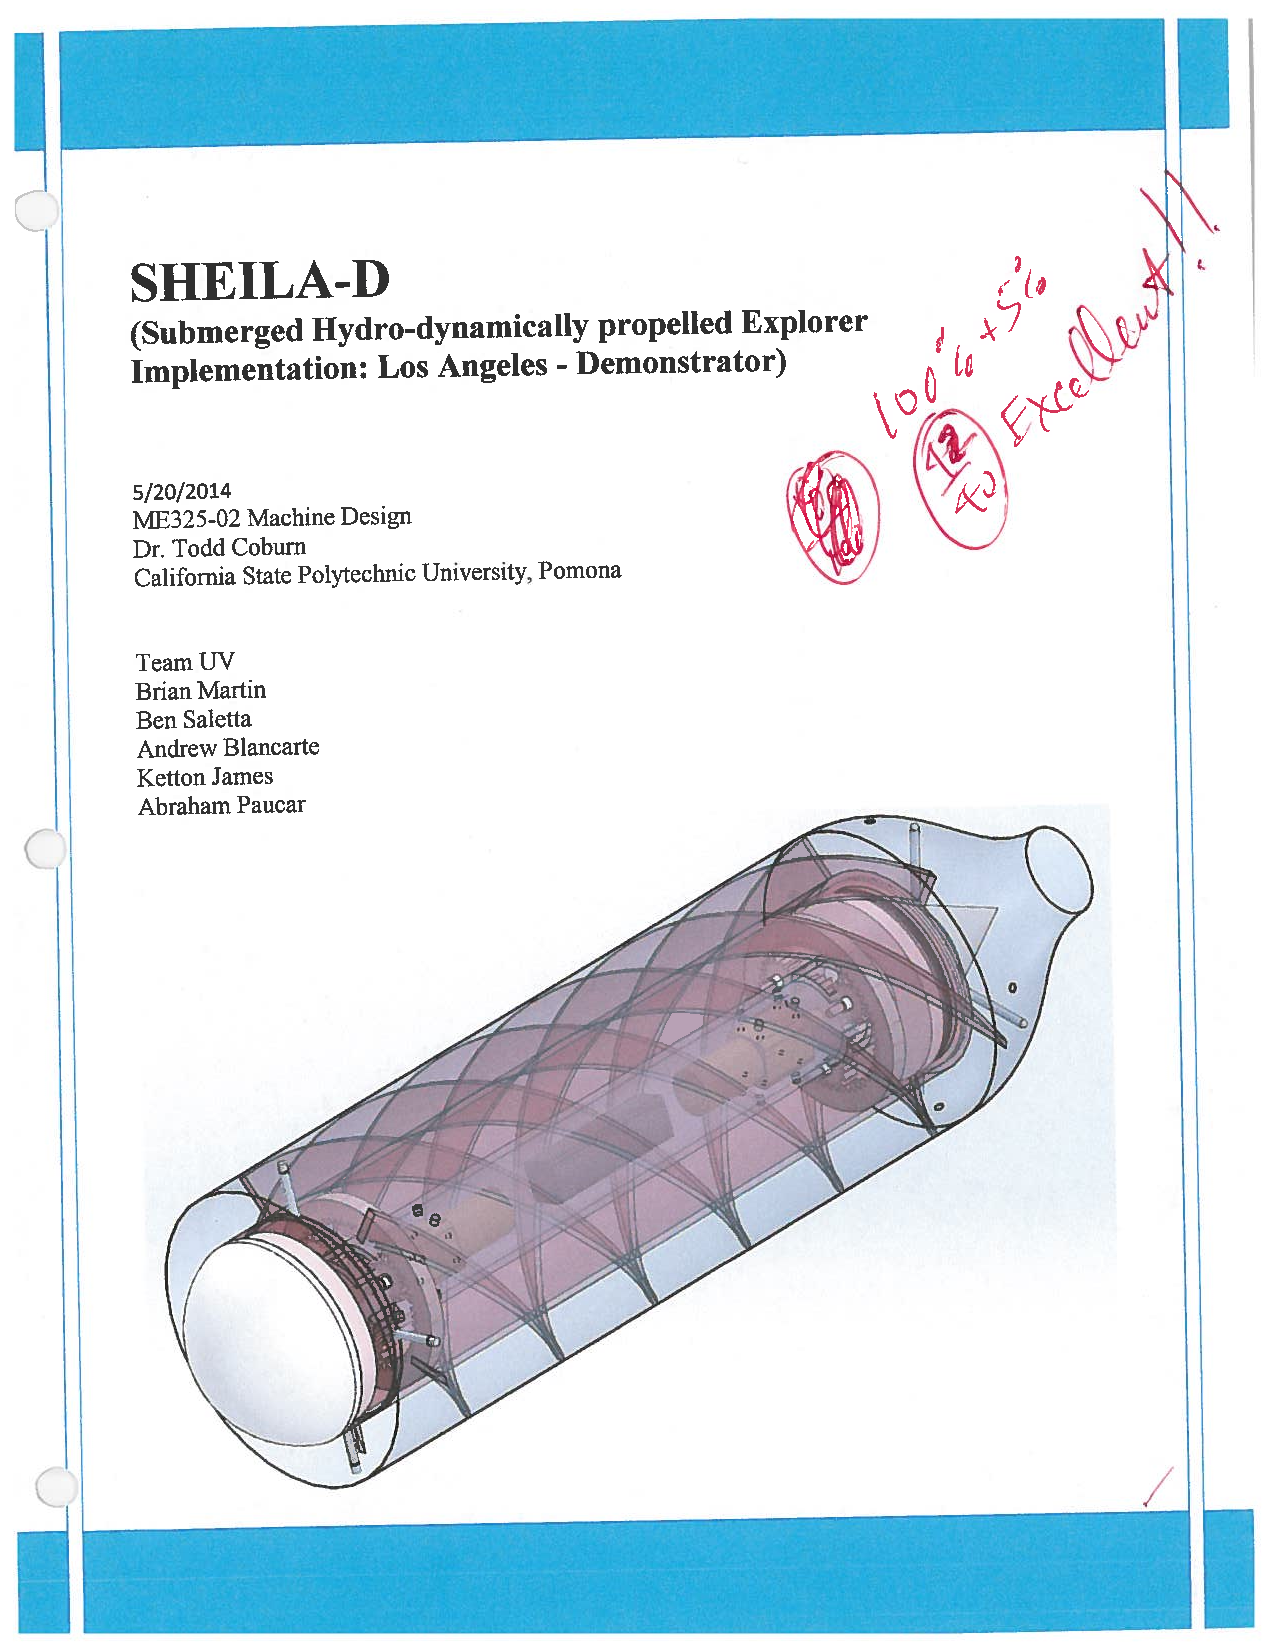
\includepdf[pages={-}]{SHEILA.pdf}
\chapter{Presentation Format}
\chapter{Electronics Data Sheets}
%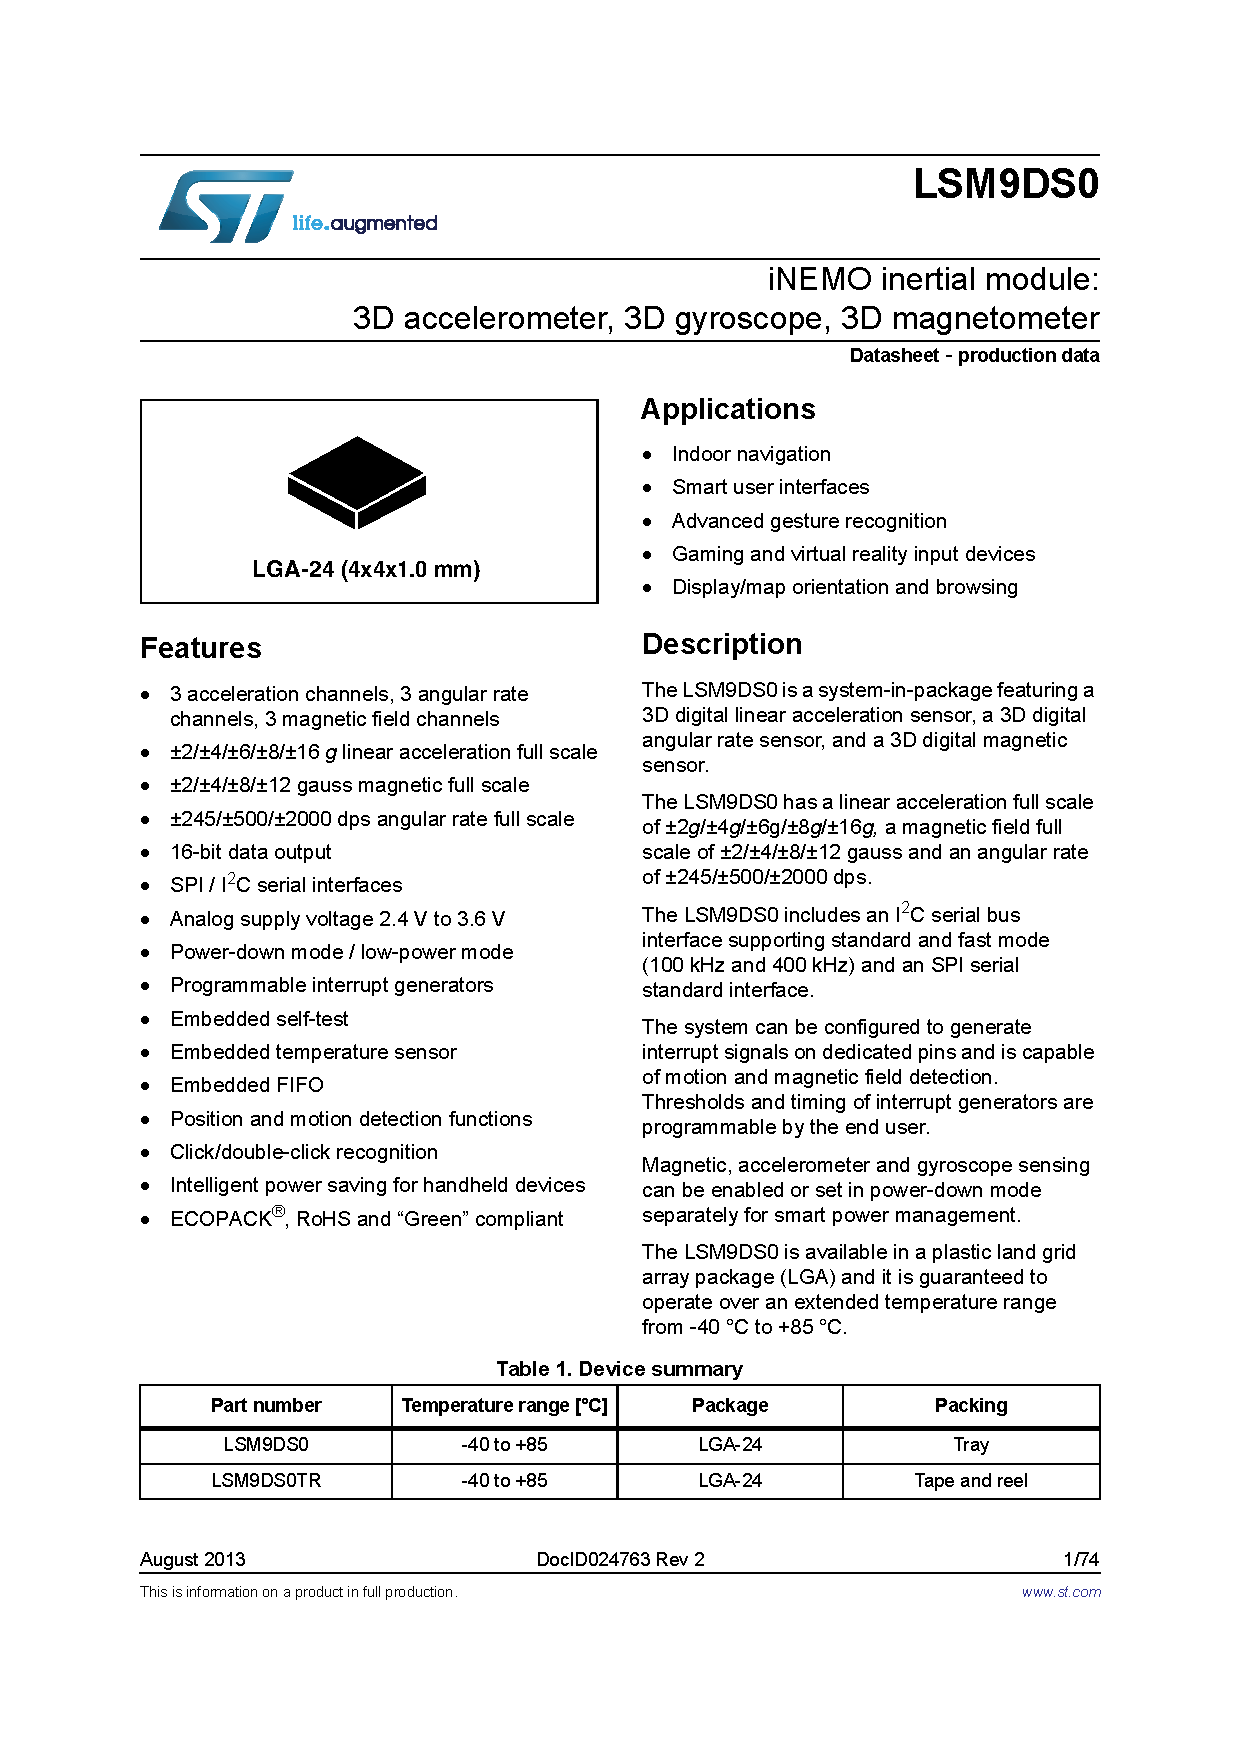
\includepdf[pages={-}]{LSM9DS0.pdf}
\begin{thebibliography}{9}
\bibitem{Rorres00}
Rorres, Chris. "The Turn of the Screw: Optimal Design of an Archimedes Screw." Journal of Hydraulic Engineering (2000): 72. Print.
\bibitem{Anderson95}
Anderson, John D. \textit{Computational Fluid Dynamics: The Basics with Applications}. New York: McGraw-Hill, 1995. Print.
\end{thebibliography}
\end{document}